
\textbf{Trabajo en el contenedor}

Se llevó a cabo un paso crucial enfocado en la preservación y durabilidad del contenedor destinado para la elaboración de este proyecto ya que, aunque se encontraba pintado, fue necesario despintar lo puesto que el recubrimiento que tenía ya presentaba algunos daños debido al traslado y el tiempo que pasó en la intemperie. Por otro lado, una vez despintado se notó que el tambo comenzaba a oxidarse.

Para contrarrestar este proceso corrosivo, se buscó adquirir una pintura que resista las altas temperaturas, esto debido a que el tambo será calentado constantemente.

Previo a pintar el tambo, se procedió a lijar aquellas partes oxidadas, una vez lijado se aplicaron dos capas de pintura, tanto por fuera, como por dentro del contenedor, obteniendo el siguiente resultado:

\begin{figure}[h!]
            \centering
            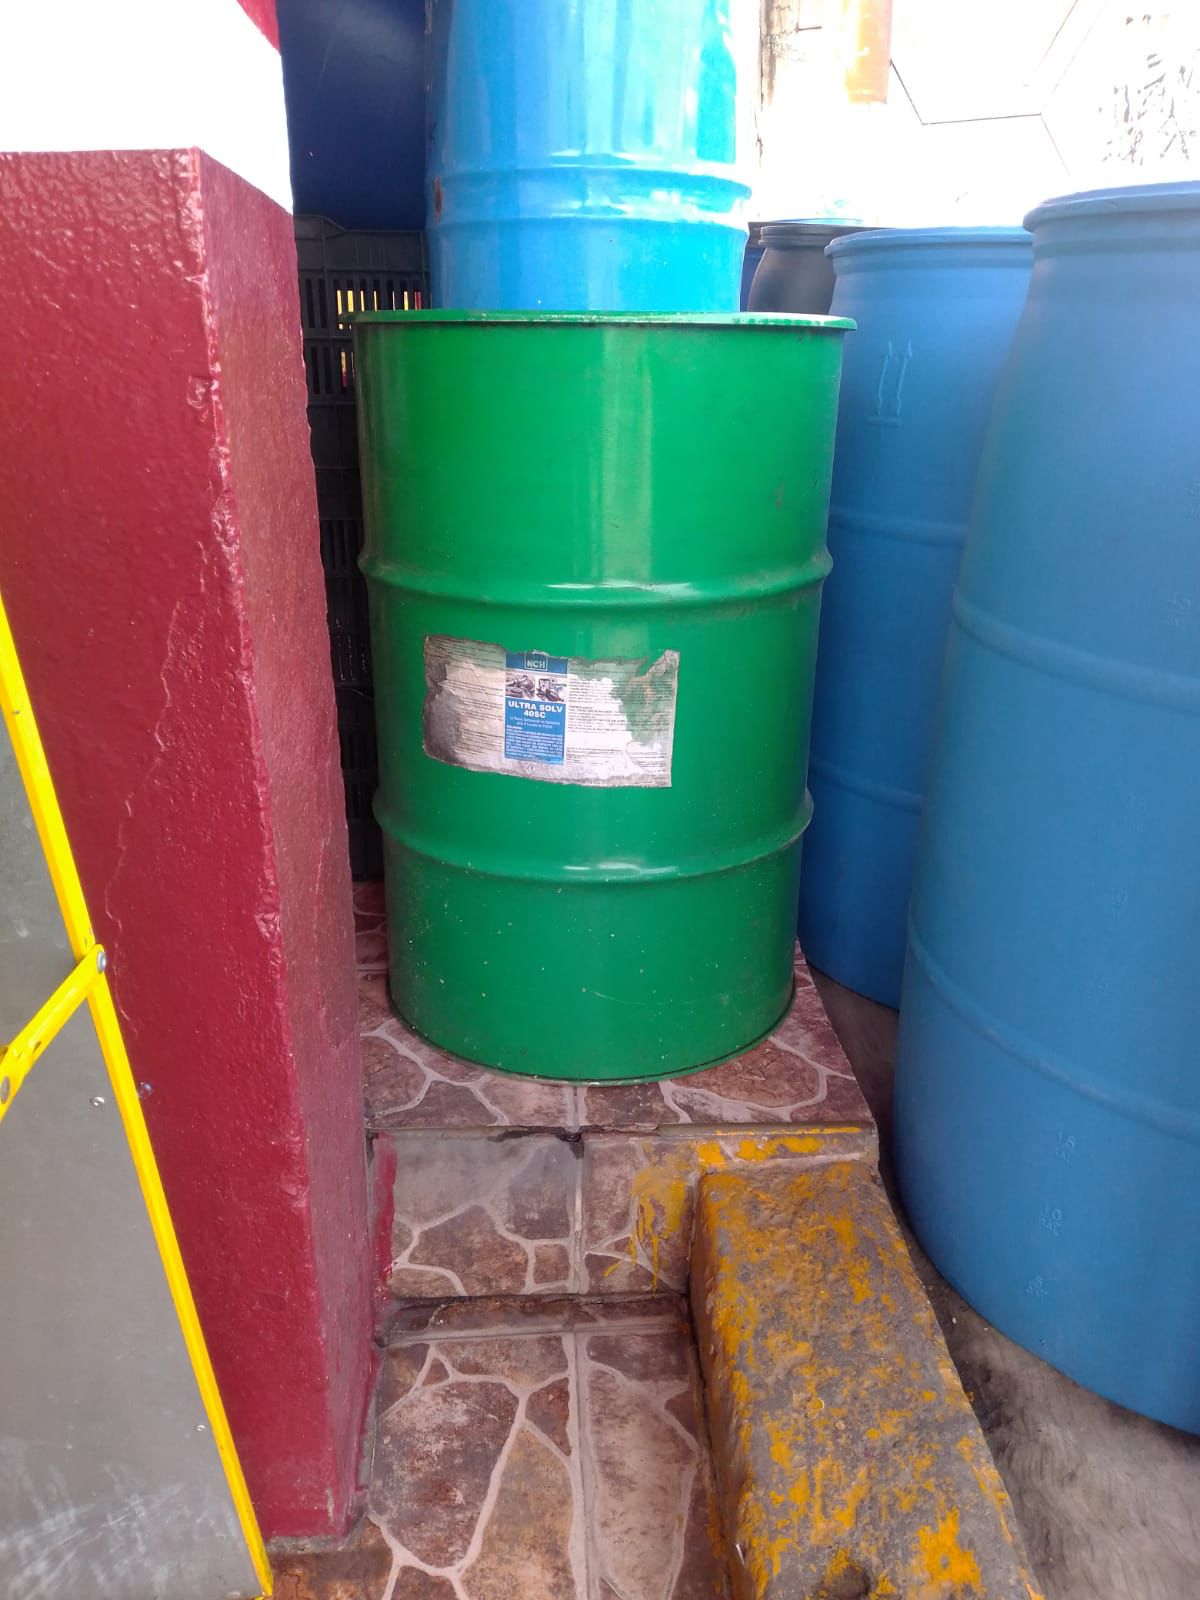
\includegraphics[scale=0.17]{images/Capitulo 4/s5/Contenedor/Contenedor_imple/contenedor_antes.jpg}
            \caption{Contenedor de acero antes}
            \label{fg:tambo_antes}
        \end{figure}
        
\newpage
\begin{figure}[h!]
            \centering
            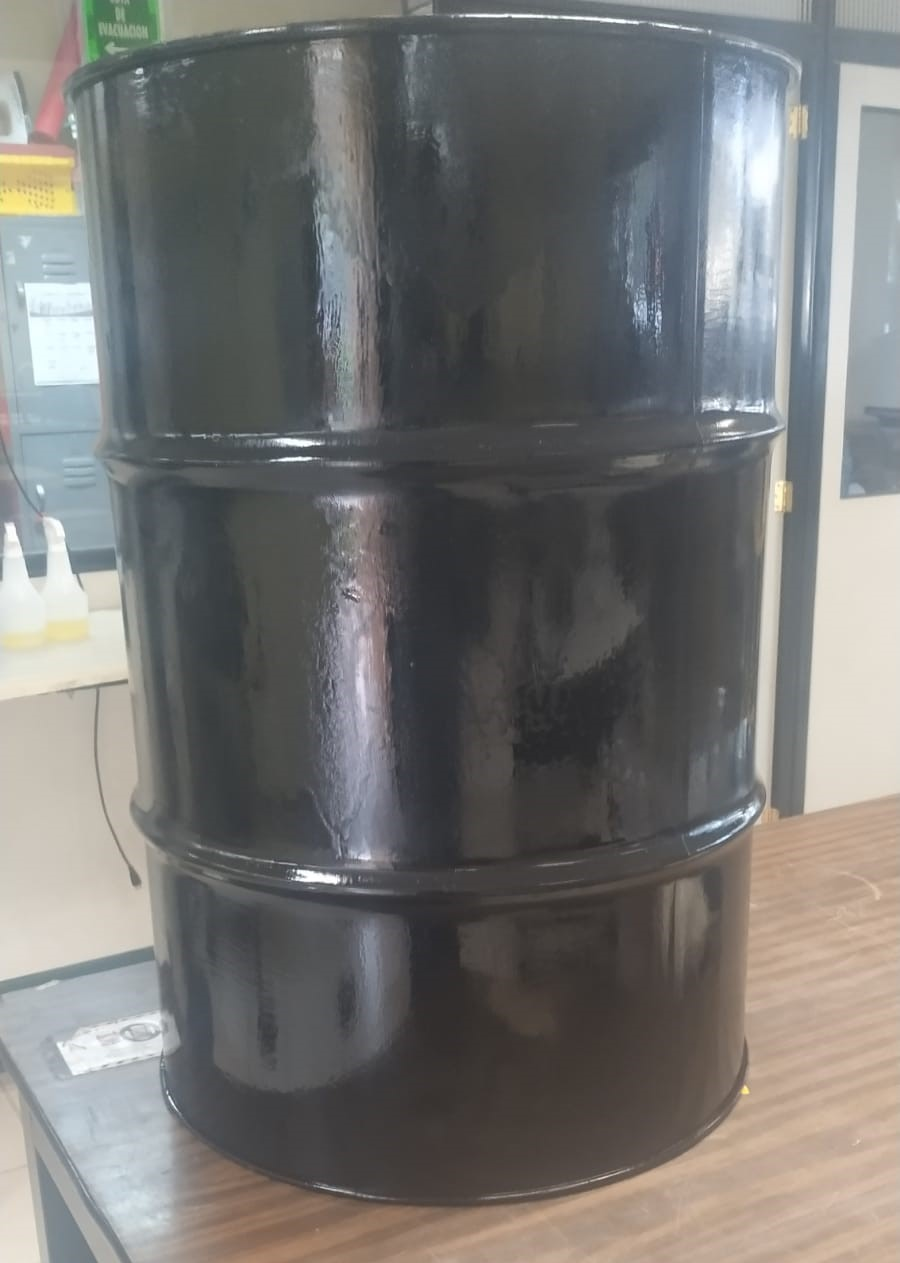
\includegraphics[scale=0.18]{images/Capitulo 4/s5/Contenedor/Contenedor_imple/contenedor_despues.jpg}
            \caption{Contenedor de acero con una capa de pintura}
            \label{fg:tambo_antes}
        \end{figure}

Posteriormente, se colocó el contenedor en la estructura y se marcaron las referencias para el paso del eje. Mediante un sacabocados se procedió a realizar las perforaciones y con ayuda de una lima se rebajó los bordes para que el eje entrara con el mínimo de juego posible.

\begin{figure}[h!]
            \centering
            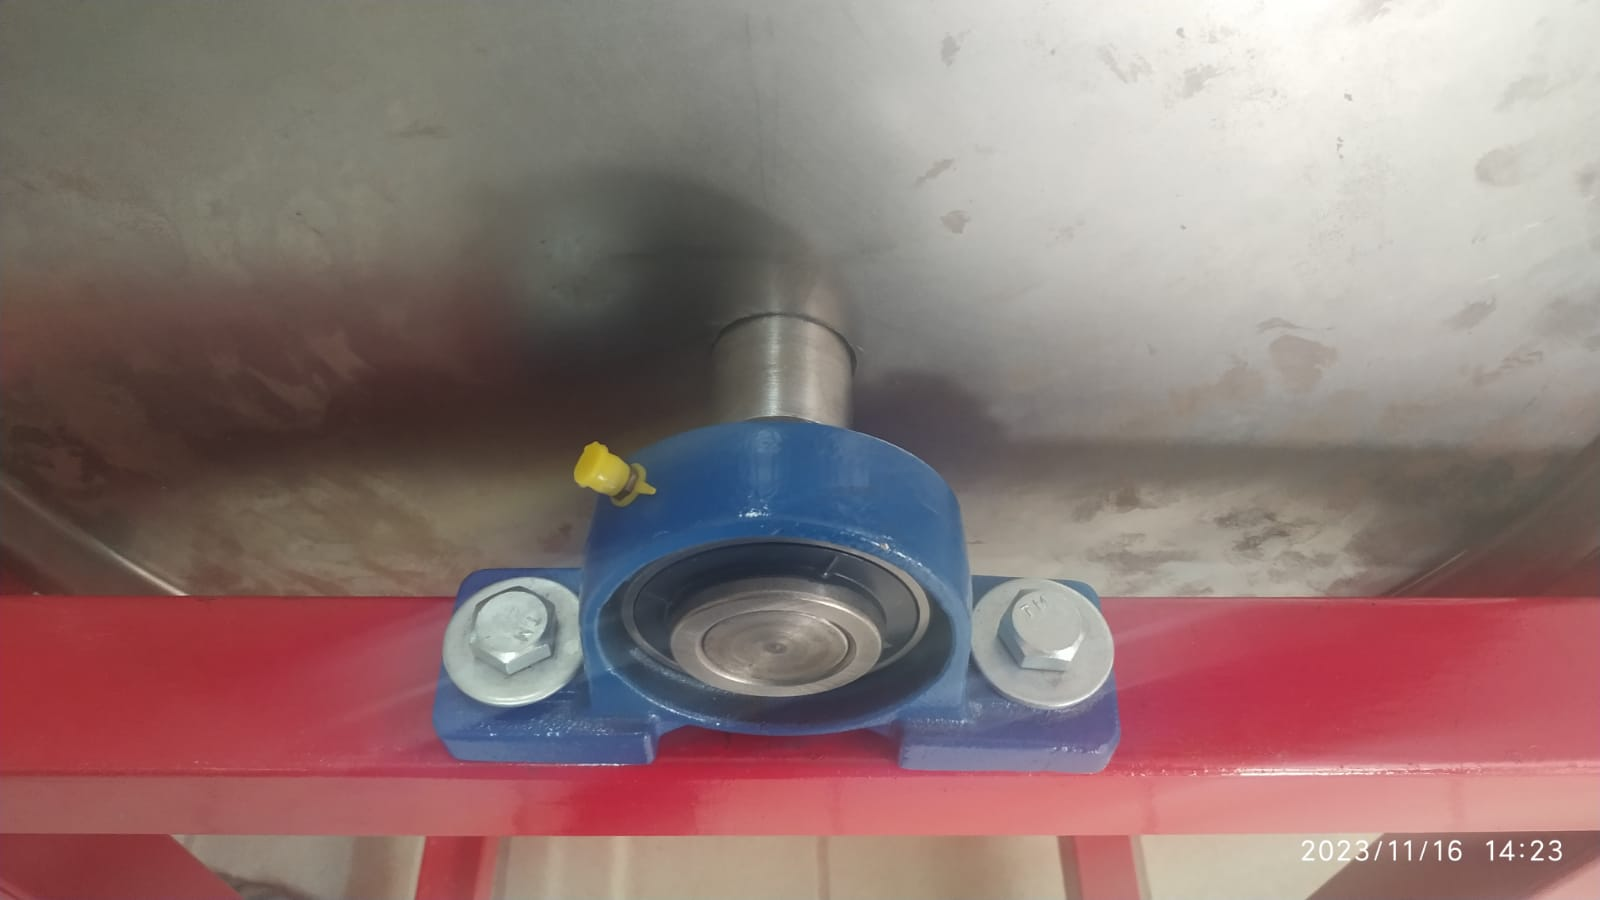
\includegraphics[scale=0.2]{images/Capitulo 4/s5/Contenedor/Contenedor_imple/tambo_montado.jpg}
            \caption{Contenedor montado en el eje}
            \label{fg:tambo_montado}
        \end{figure}
        \newpage
\textbf{Sistema de autorregulación de temperatura
}
Para la implementación de este sistema, se realizó un gran ajuste. Debido a los riesgos que implicaban tener las resistencias eléctricas expuestas, tales como quemaduras y riesgo de un corto circuito, además de su muy baja eficiencia, se optó por revisar otras soluciones disponibles en el mercado. 

De esta manera, se llegó a la conclusión de utilizar un cinturón especial para calentamiento de tambos de aceite, como el de la figura \ref{fg:cinturon_calentador}.  Este dispositivo si es mas caro a comparación de las resistencias, pero nos ofrece mayor seguridad, cubriendo las resistencias 

\begin{figure}[h!]
            \centering
            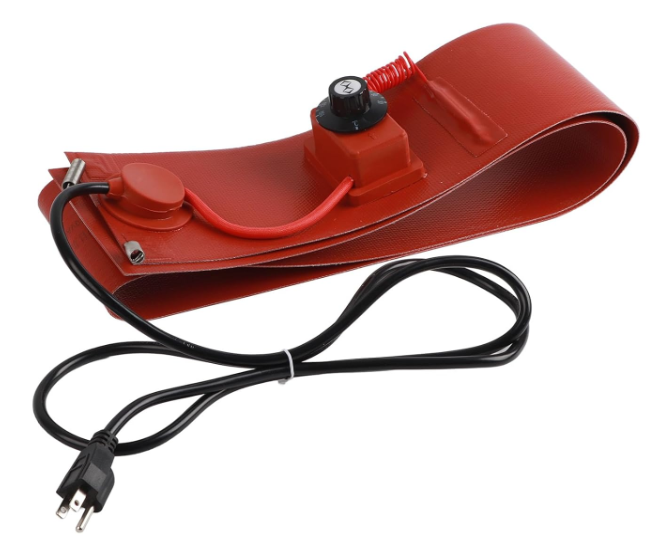
\includegraphics[scale=0.2]{images/Capitulo_Imple/S5/Actuadores/calentador.png}
            \caption{Cinturón calentador de tambos}
            \label{fg:cinturon_calentador}
        \end{figure}
        Este sistema rodea la parte central del tambo, estará directamente configurado para calentar la pared del contenedor a una temperatura de $100 °C$ y estará controlado por medio de un controlador "On/OFF" que sera el encargado de encenderlo únicamente cuando sea necesario.

        En las pruebas que se realizaron, se comprobó que es capas de transmitir el calor al interior a la materia dentro del contenedor, llegando a una temperatura de $75 °C$ en aproximadamente 10 minutos. Además de solo consumir un $1 Kw/hr$ de energía.
        
\textbf{Sistema de ventilación}

Para este sistema fue necesario diseñar una pieza que permita conectar la salida del contenedor, a la entrada del filtro, dada la forma del contenedor resultaba imposible colocarlo directamente.
Se procedió a diseñar la pieza en SolidWorks en donde se obtuvo el siguiente resultado:

\begin{figure}[h]
            \centering
            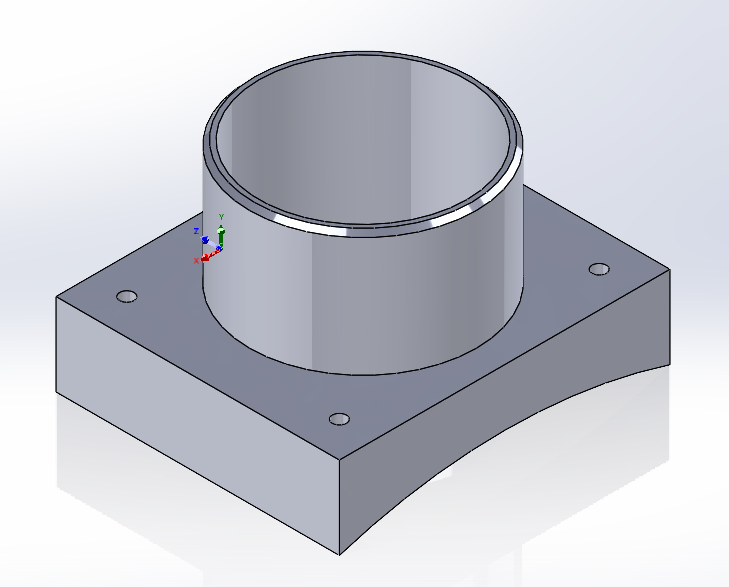
\includegraphics[scale=0.35]{images/Capitulo 4/s5/Contenedor/Contenedor_imple/adaptador_filtro.png}
            \caption{Adaptador para filtro}
            \label{fg:adap_filtro}
 \end{figure}

Dado que la pieza presenta una geometría bastante particular, la mejor opción fue imprimirla en 3D. Se procedió a ajustar algunos detalles previo a la impresión, teniendo un estimado de 13 horas para le impresión total de la pieza.

\begin{figure}[h]
            \centering
            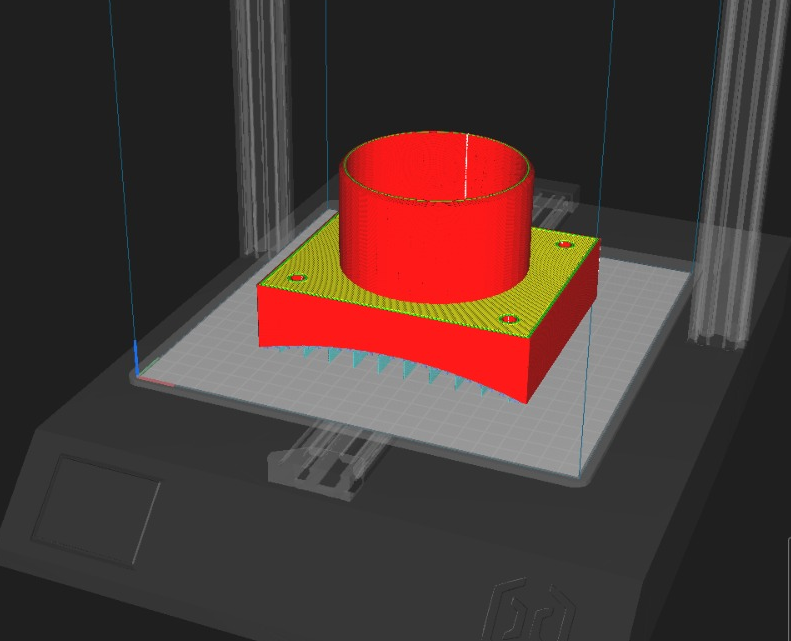
\includegraphics[scale=0.32]{images/Capitulo 4/s5/Contenedor/Contenedor_imple/imp_filtro_1.png}
            \caption{Ajuste de parámetros software de impresión}
            \label{fg:impresion_filtro1}
 \end{figure}
 \newpage
Posteriormente se realizó el proceso de impresión obteniendo:
\begin{figure}[h]
            \centering
            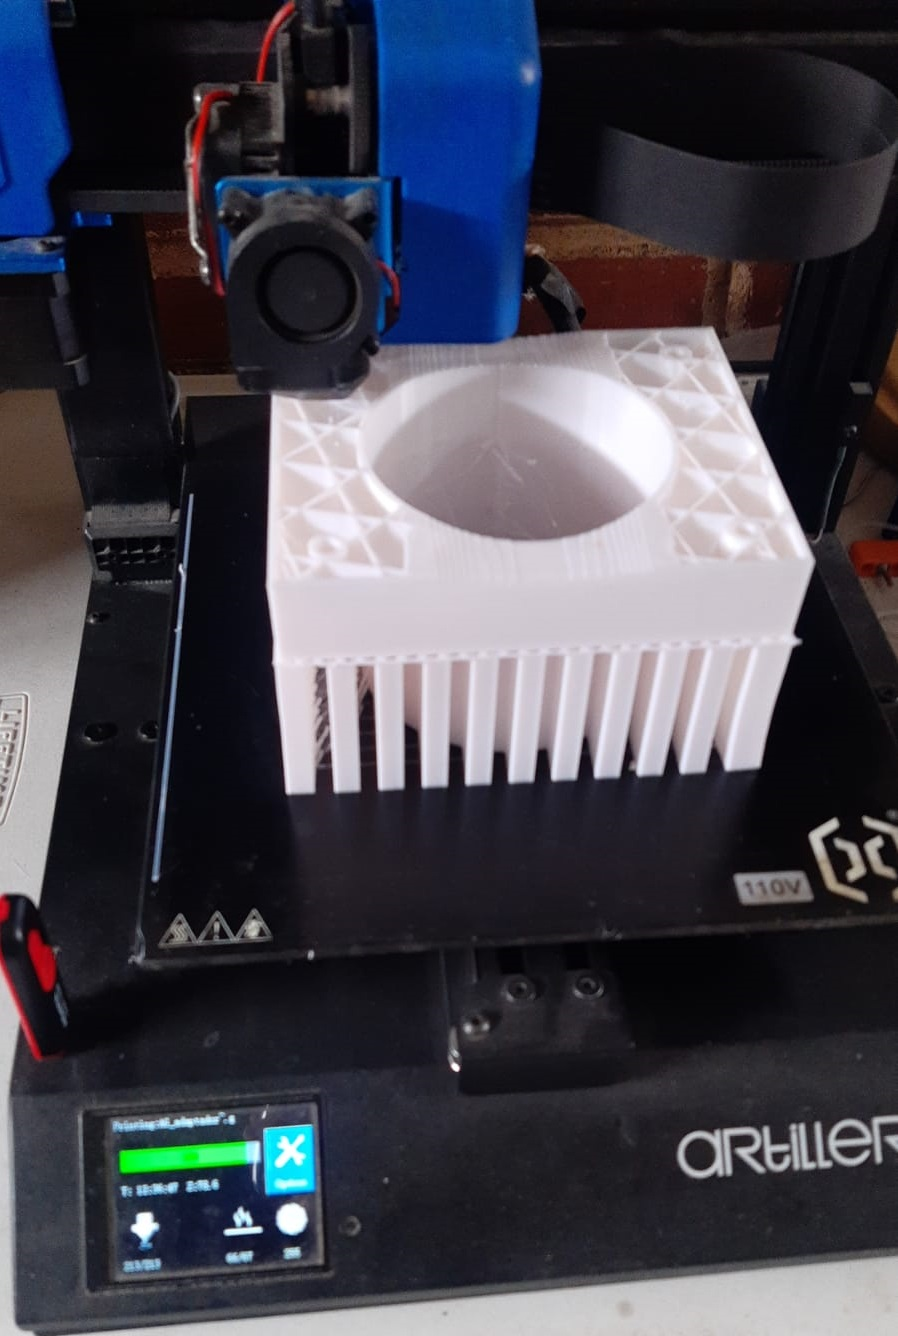
\includegraphics[scale=0.18]{images/Capitulo 4/s5/Contenedor/Contenedor_imple/imp_filtro_2.jpg}
            \caption{Impresión 3D adaptador para filtro}
            \label{fg:impresion_filtro2}
 \end{figure}

 Una vez impresa la pieza, se retiraron los soportes que coloca la impresora para que la pieza no pierda su forma y se procedió a colocar la pieza en el contenedor, se realizaron algunos barrenos en el tambo para poder fijarla.

 \begin{figure}[h]
            \centering
            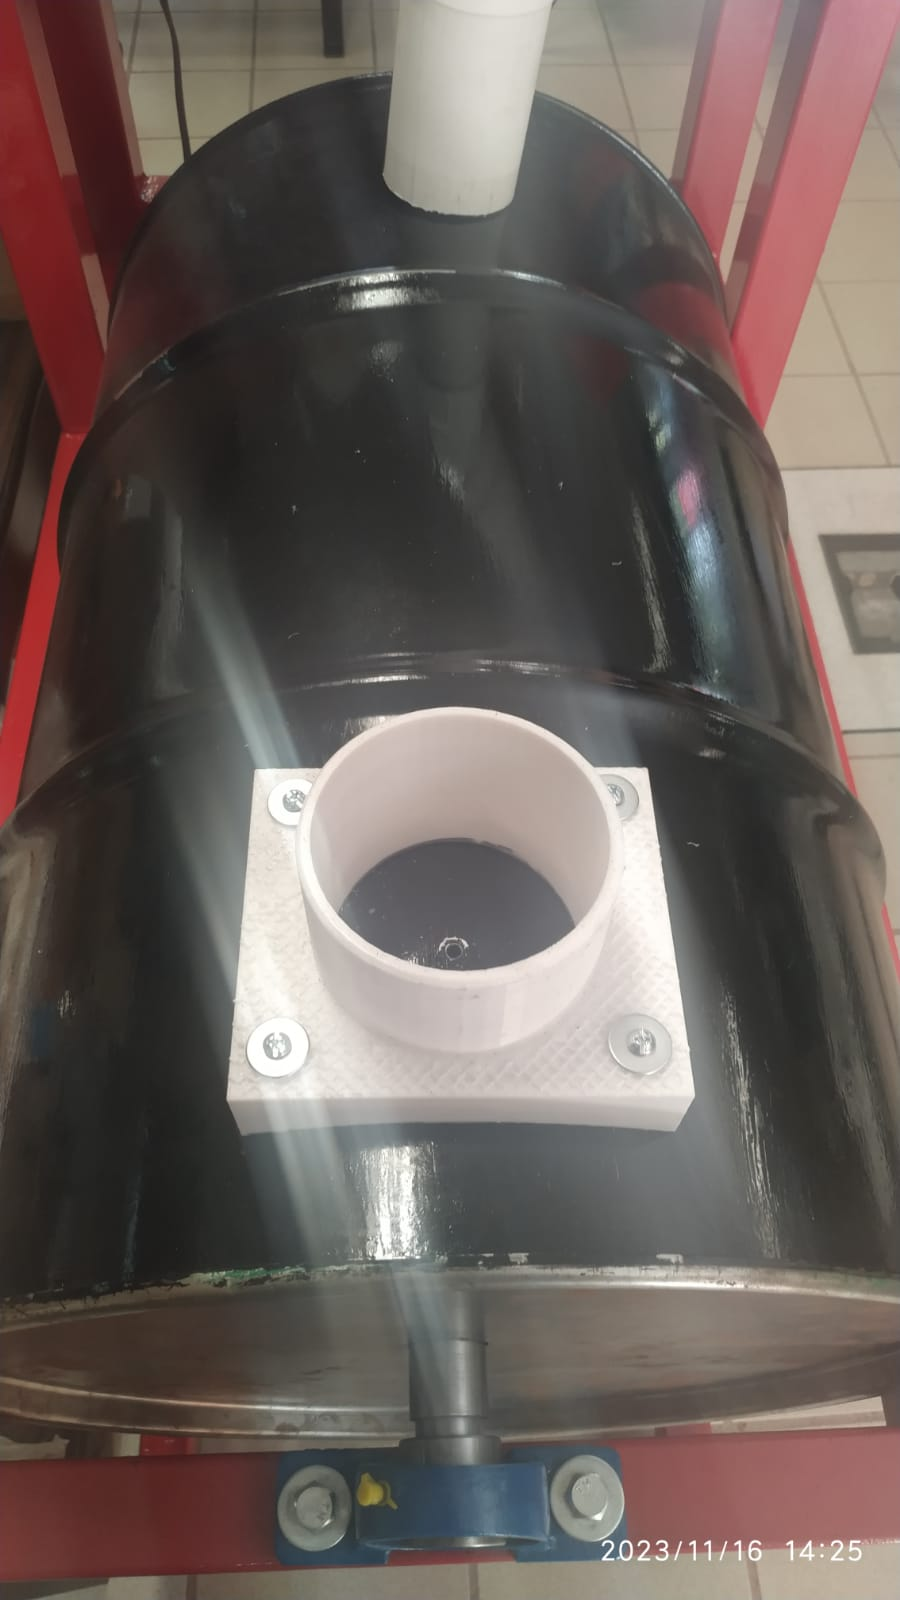
\includegraphics[scale=0.1]{images/Capitulo 4/s5/Contenedor/Contenedor_imple/adaptadorfilt_montado2.jpg}
            \caption{Adaptador montado en el contenedor}
            \label{fg:adaptador_montado_tambo}
 \end{figure}

 \newpage
 \begin{figure}[h]
            \centering
            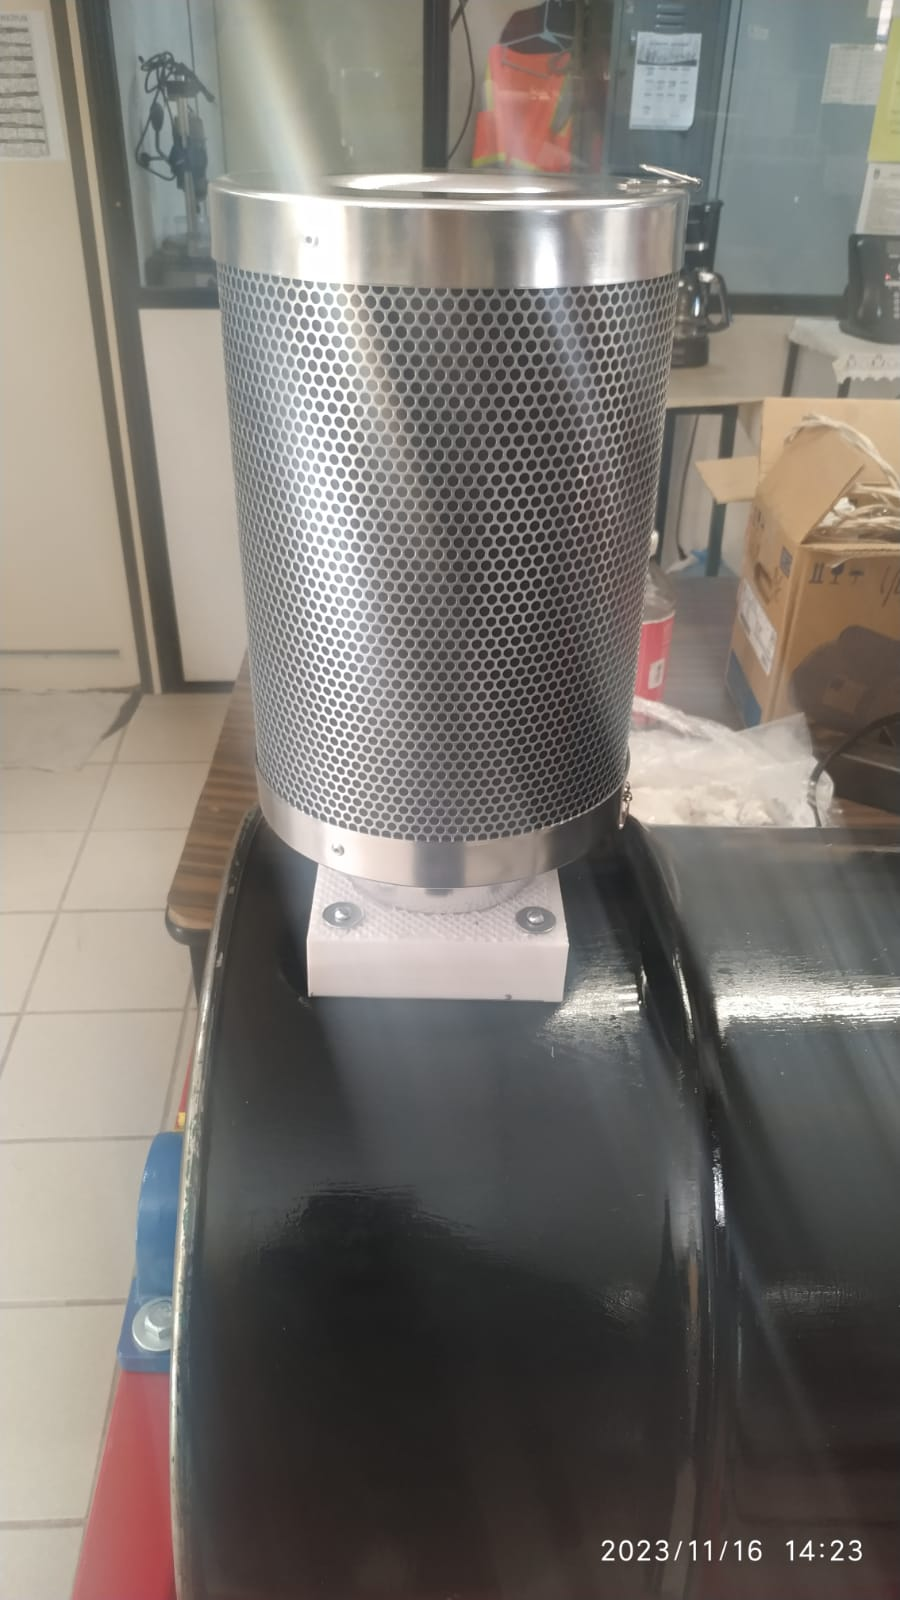
\includegraphics[scale=0.15]{images/Capitulo 4/s5/Contenedor/Contenedor_imple/adaptadorfilt_montado.jpg}
            \caption{Adaptador ensamblado con filtro}
            \label{fg:adaptador_filtro_montados}
 \end{figure}
Para facilitar la entrada de aire al contenedor, se empleó un ventilador de computadora de 3'', por lo que fue necesario diseñar una pieza que permitiera enlazarlo a la estructura de PVC, en consecuencia se modeló una base para el ventilador en SolidWorks, esta pieza fue impresa en 3D obteniéndose el siguiente resultado:
 \begin{figure}[h]
            \centering
            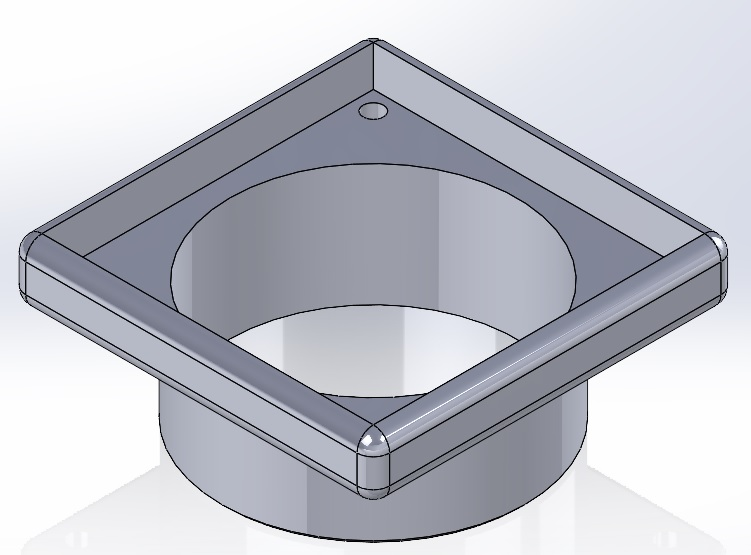
\includegraphics[scale=0.15]{images/Pruebas_S5/pieza_ventilador.jpg}
            \caption{Diseño adaptador para ventilador en SolidWorks}
            \label{fg:adaptador_ventilador}
            
 \end{figure}
  \begin{figure}[h]
            \centering
            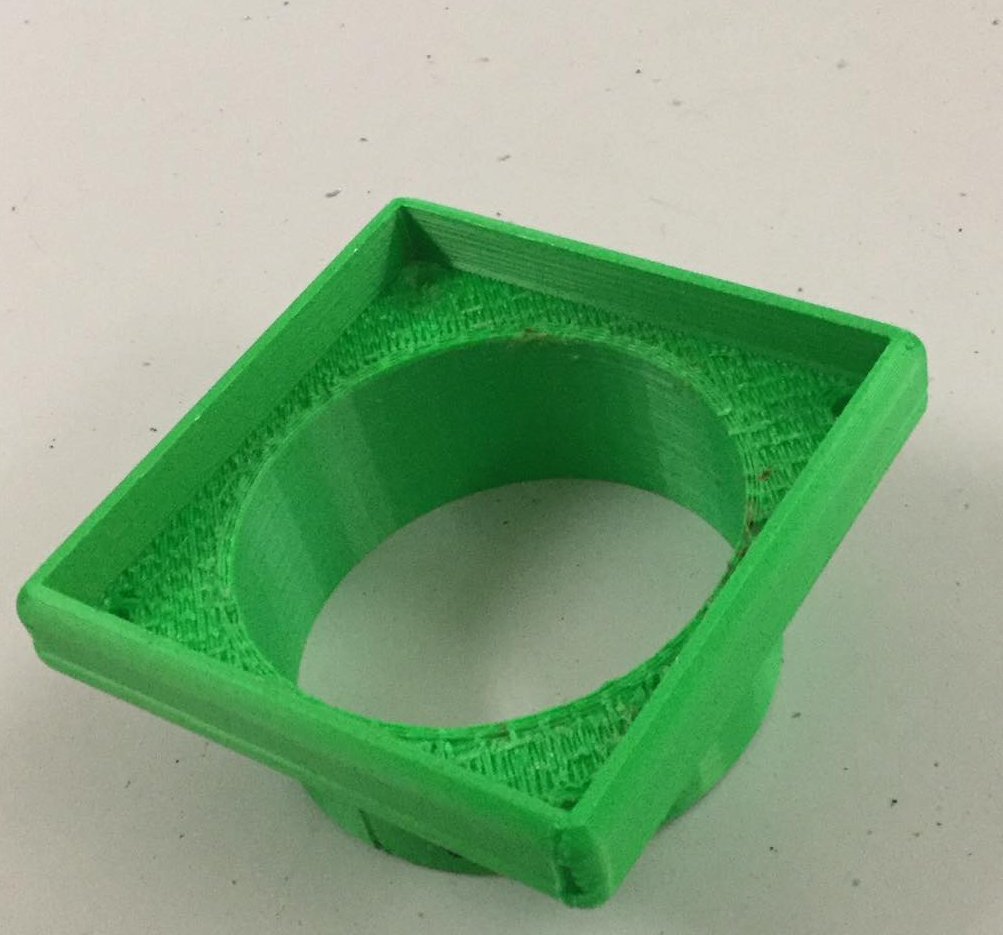
\includegraphics[scale=0.15]{images/Pruebas_S5/pieza_ventilador_impresa.png}
            \caption{Impresión 3D adaptador para ventilador}
            \label{fg:adaptador_ventilador}
            
 \end{figure}
\textbf{ Sistema de aireación}

 Para el sistema de aireación, se realizó la manufactura del eje a partir de un tajo de acero, el cual se manipuló a través de un torno, aplicando las operaciones de careado, cilindrado y desbaste para generar cada una de las secciones funcionales del eje.

 Este elemento tiene un diámetro de $1 \frac{1}{2} in$ por lo que fue necesario conseguir las chumaceras de esta medida para sostener el eje el la estructura y a su vez permitirle girar sin riesgo de fricción.

 En uno de los extremos del eje, se coloco una polea, la cual esta fijada con un esclavo, un anillo de acero y una chaveta para transmitir el movimiento proveniente de un motor de corriente alterna de $\frac{1}{4} Hp$. 

 El motor esta conectado a una reductor de $\frac{1}{40}$ y tiene una polea de salida $2 \frac{1}{2} in$
 por lo que se al final, el eje estará girando a una velocidad de 6 $rpm$, velocidad suficiente para realizar el proceso de aireación y mezcla de los desechos a su interior (Figura \ref{fg:montaje airo}.

 También ofrece el momento necesario para poder voltear los 20 $kg$ de materia que se pretenden procesar en su interior.

 Este motor eléctrico es activado por medio de una señal que sale de la ESP32, el cual abre la señal para la activación de un contactor eléctrico, el cual es capaz de soportar la corriente de arranque del motor eléctrico y de esta forma, se puede llevar a cabo el proceso de aireación de forma automática.

  \begin{figure}[h]
            \centering
            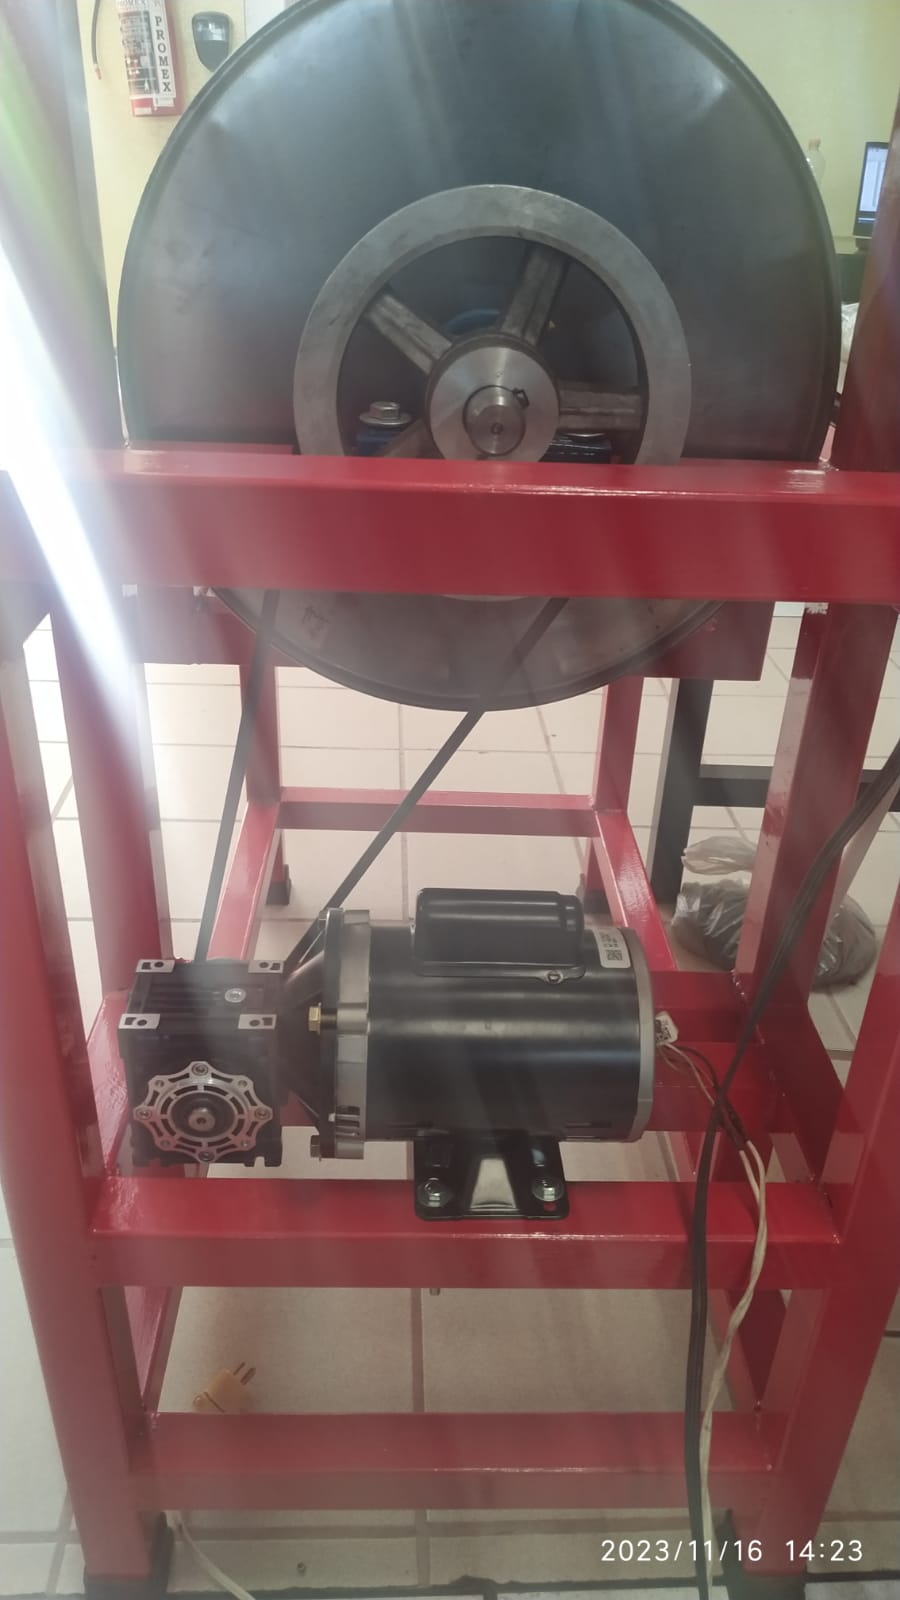
\includegraphics[scale=0.2]{images/Capitulo_Imple/S5/Aireacion.jpeg}
            \caption{Montaje del sistema de aireación}
            \label{fg:montaje airo}
 \end{figure}
 Para la construcción del sistema de palas, se utilizaron secciones de tubo con cuerda, a las que por medio de un esmeril se les retiró parte de la cuerda dejándolos como tubos lisos. 
 Posteriormente  se cortaron rectángulos de (medidas ***) de un pedazo de tubo rectangular para la fabricación de las palas, se optó por esa disposición de palas debido a que era necesario revolver de manera uniforme toda la mezcla, y que la formación de surcos podría afectar a la mezcla. 
 El tamaño y disposición de las palas, garantiza que no queden surcos y que toda la materia se mezcle de manera uniforme, lo que en consecuencia permite que el calor se distribuya de manera uniforme en toda la mezcla al igual que al momento de oxigenar.

 Una vez cortadas las palas, se procedió a soldarlas a las secciones de tubo con cuerda, obteniendo el siguiente resultado:

   \begin{figure}[h]
            \centering
            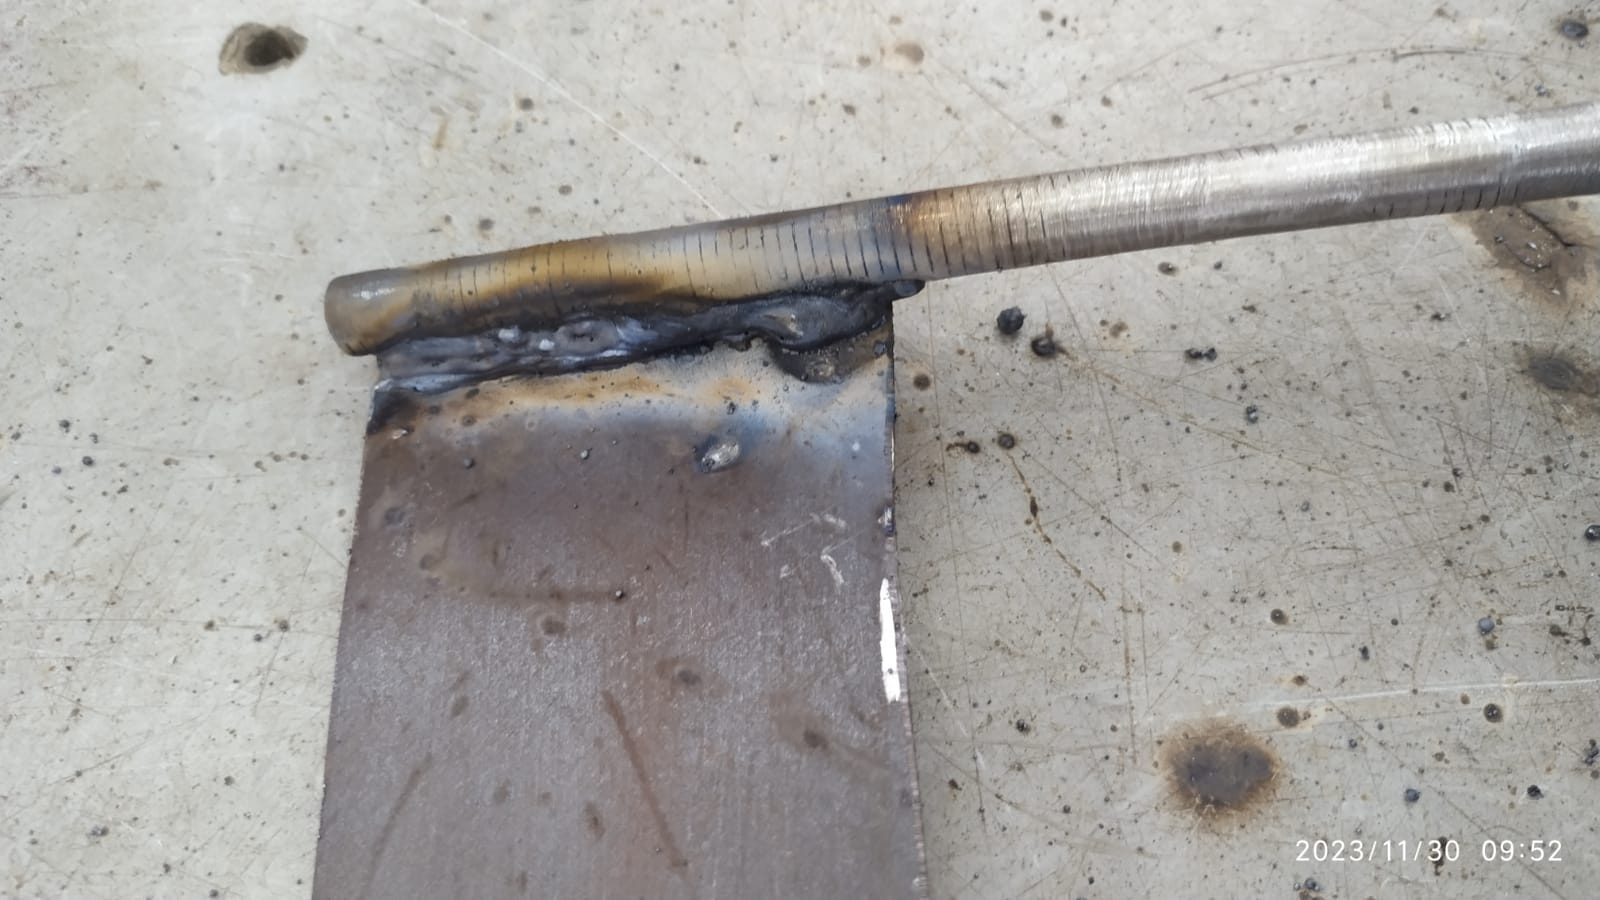
\includegraphics[scale=0.2]{images/Pruebas_S5/pala_soldada.jpeg}
            \caption{Pala soldada a sección de tubo con cuerda}
            \label{fg:soldar_pala}
 \end{figure}


Por último fue necesario realizar un aplanamiento de secciones en el eje  empleando una fresadora. Esto con el fin de facilitar la sujeción de las palas al eje. (Figura \ref{fg:eje_fresado})  

\begin{figure}[h!]
            \centering
            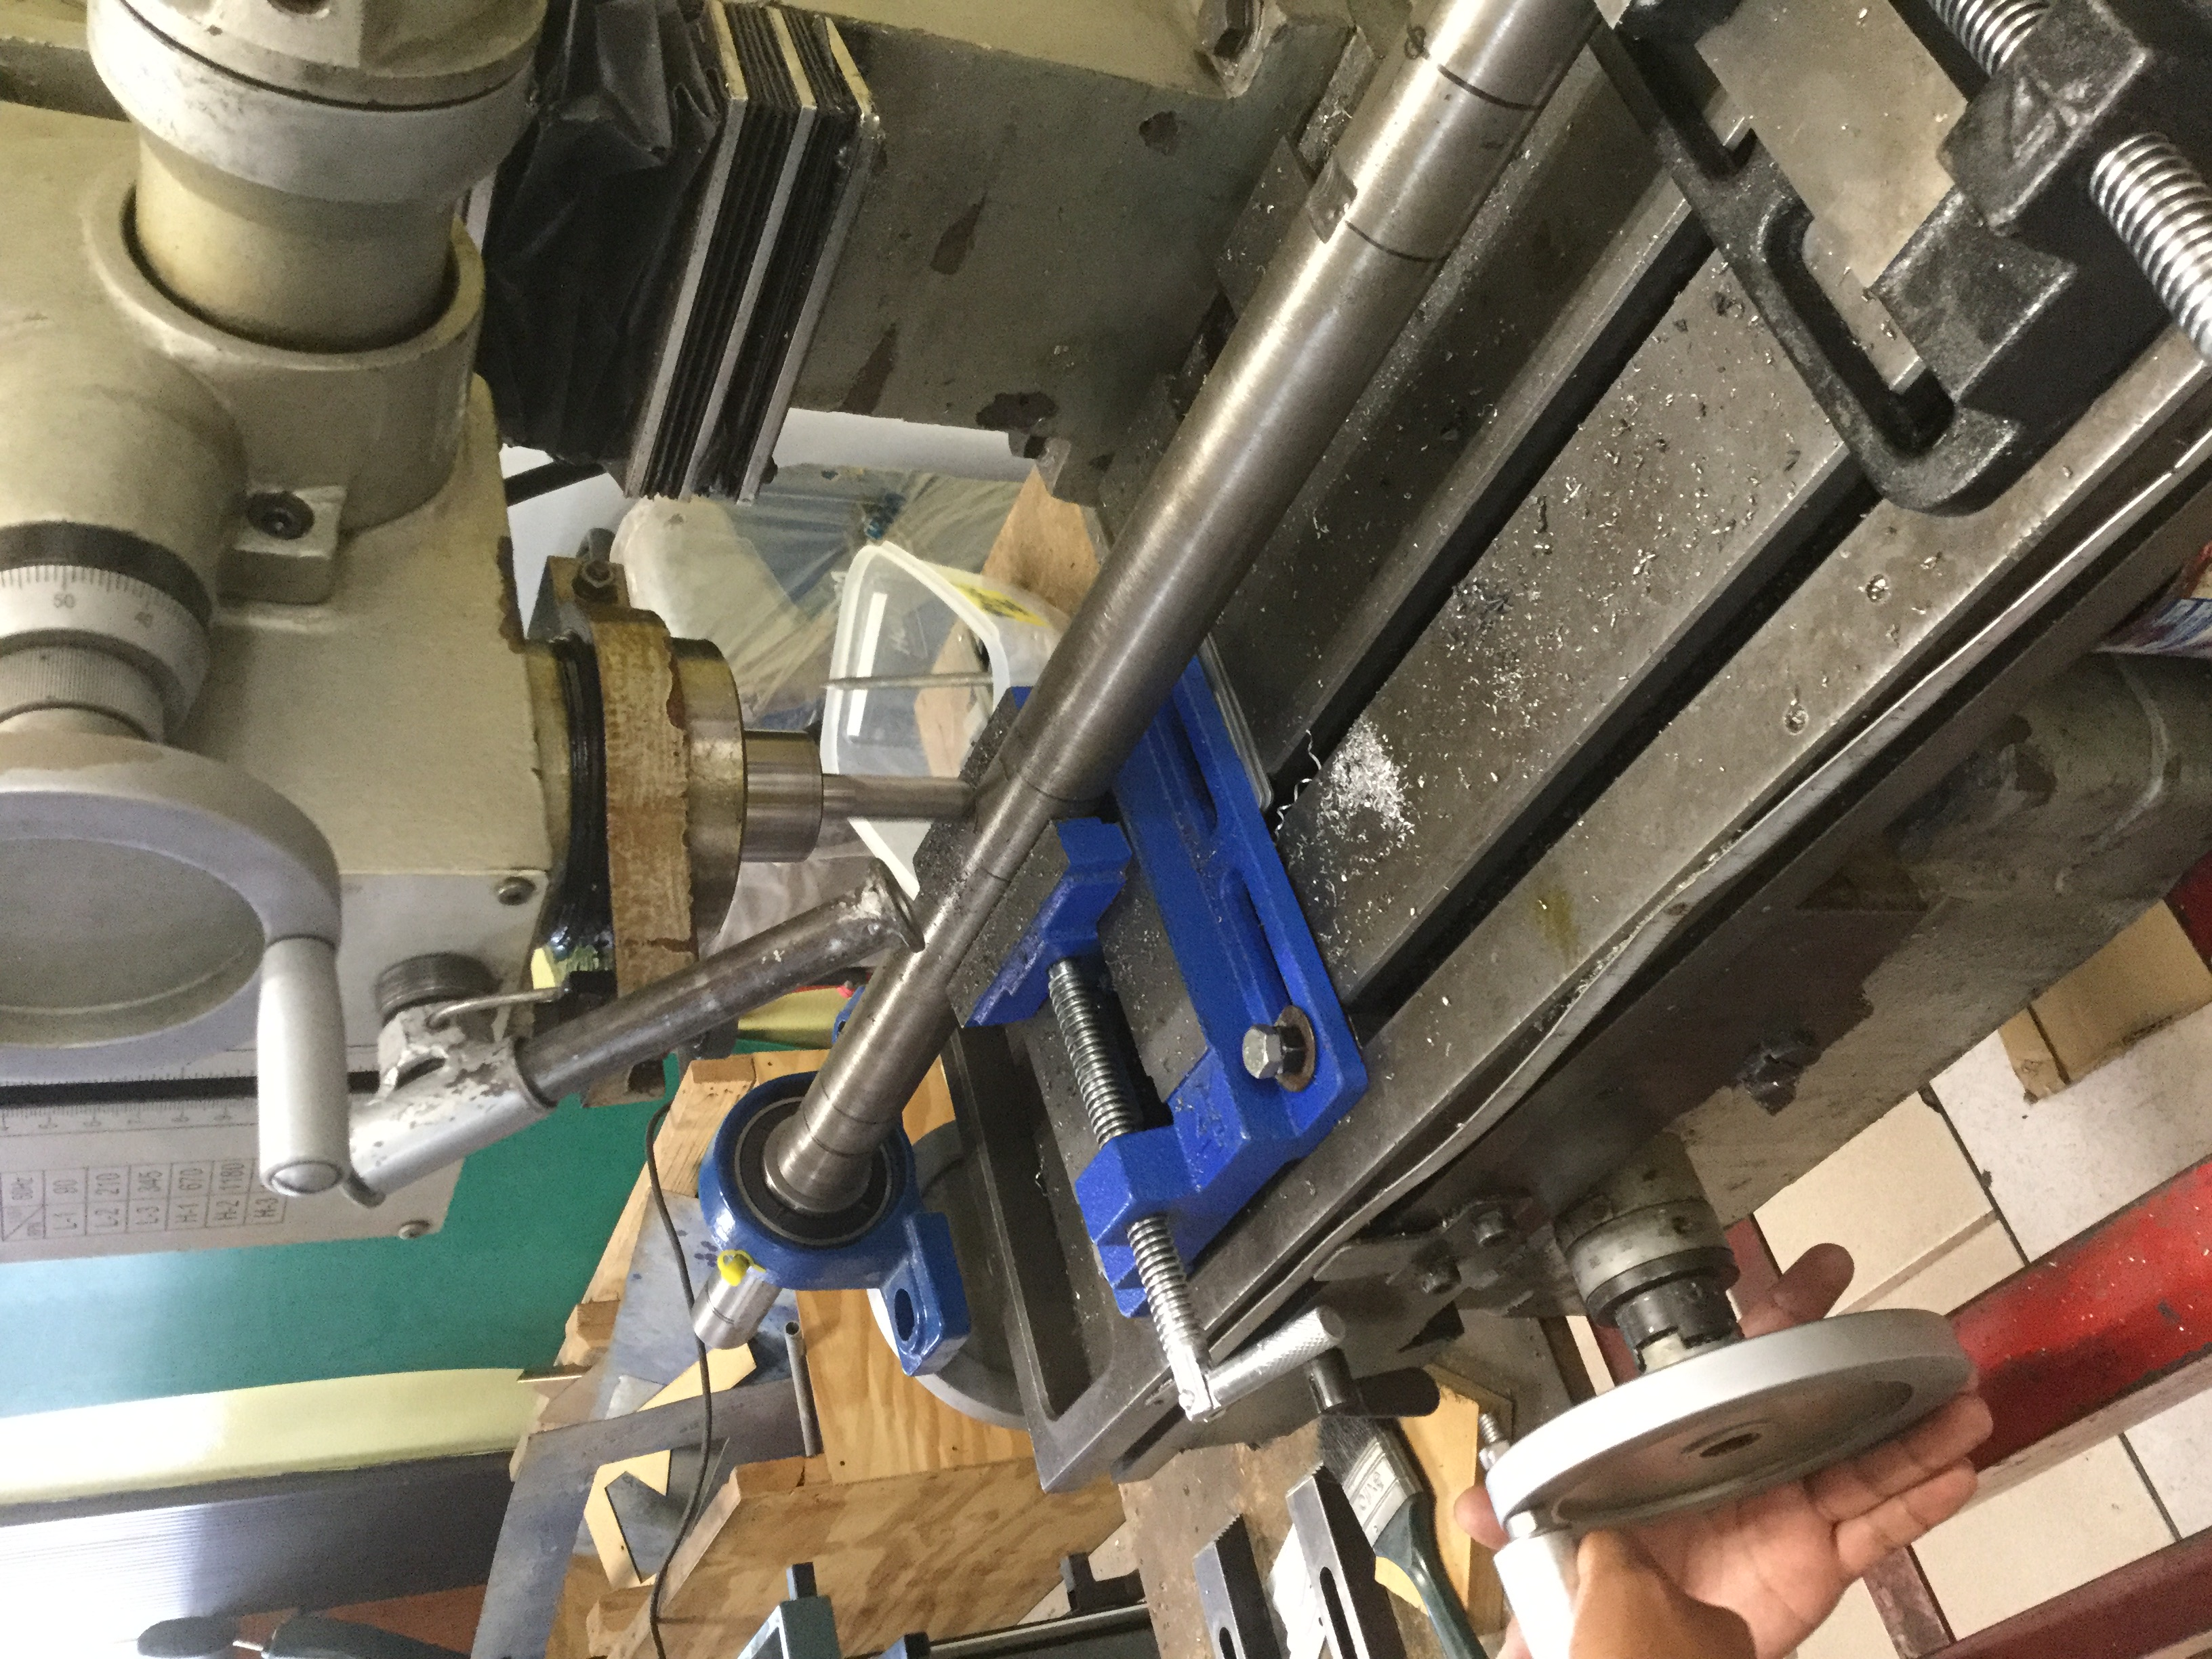
\includegraphics[scale=0.09, angle=270]{images/Capitulo_Imple/S5/fresado.JPG}
            \caption{Proceso de fresado del eje}
            \label{fg:eje_fresado}
        \end{figure}

\textbf{Aislamiento térmico}
Por medio de fibra de vidrio se forró todo el contenedor,  realizando los cortes pertinentes para la salida al filtro, al sistema de triturado y  el cable del cinturón. Para esta parte se colocaron los diversos componentes en su lugar para tomar medidas y realizar los cortes. (Figura \ref{fg:tambo_sin_cubir})

\begin{figure}[h!]
            \centering
            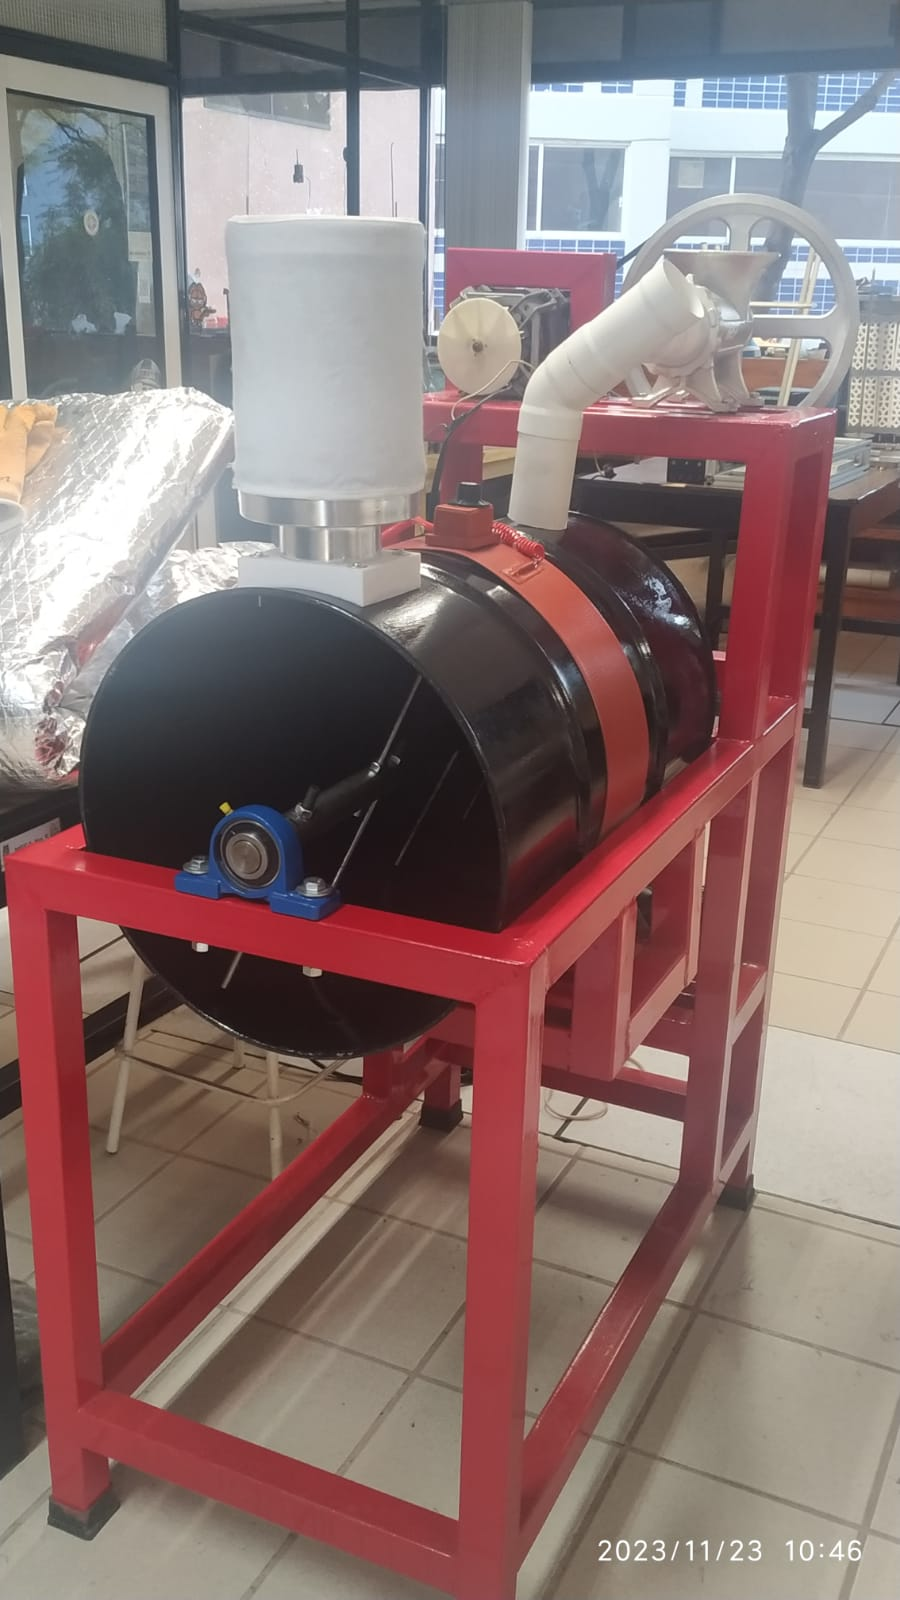
\includegraphics[scale=0.15]{images/Capitulo_Imple/S5/tambo_sin_cubrir.jpeg}
            \caption{Instalación de los elementos del tambo sin recubrimiento}
            \label{fg:tambo_sin_cubir}
        \end{figure}

Para sujetar la fibra, se utilizó una cinta perforada de aluminio, la cual se sujetó con un tornillo y una tuerca. (Figura \ref{fg:tambo_cubierto}).

\begin{figure}[h!]
            \centering
            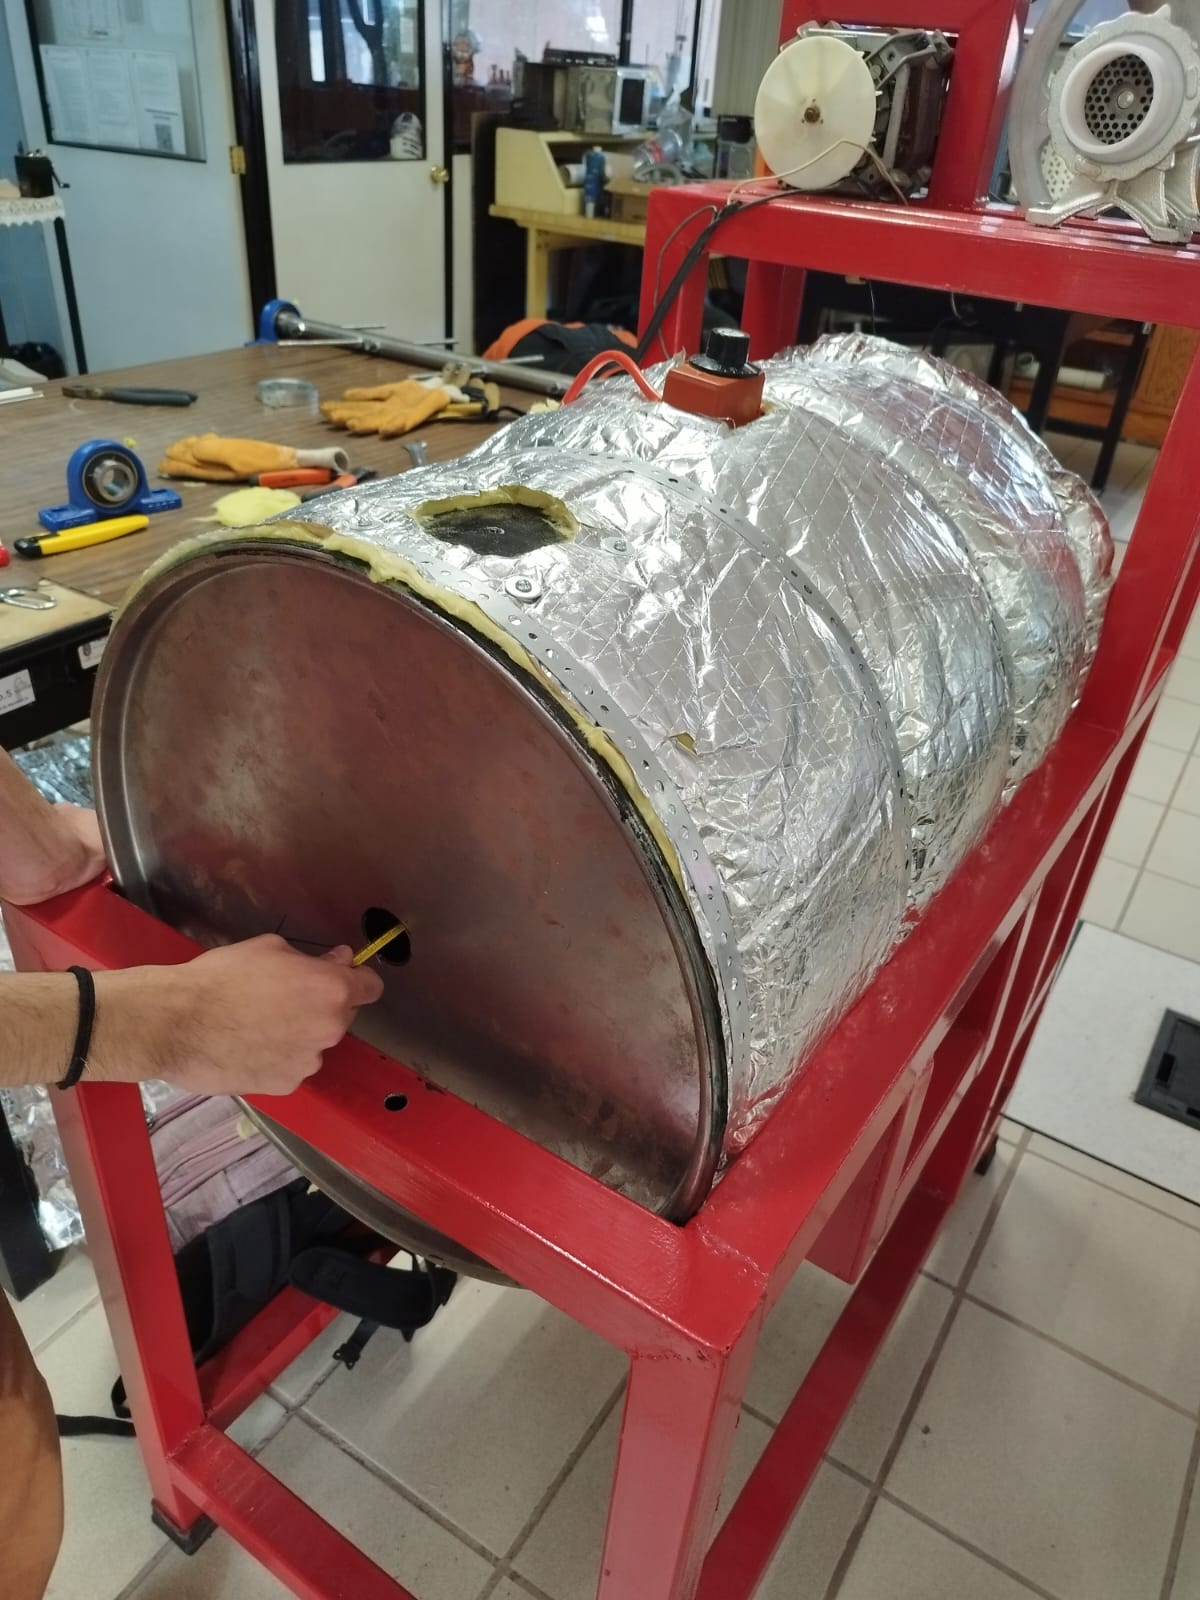
\includegraphics[scale=0.18]{images/Capitulo_Imple/S5/tambo_solo.jpeg}
            \caption{Contenedor con el recubrimiento instalado}
            \label{fg:tambo_cubierto}
        \end{figure}